\section{Computer Design}

As good computer engineers, we ought to study computer
design so we can design new computers and understand
the ones that already exist.

In this class, we generally represent numbers in
binary, or more commonly, hex. Converting from
hex to binary is simple: take each hex digit, convert
it to its corresponding binary representation, and
insert that in the corresponding space in the binary
number. For example, \texttt{0xeca8} becomes
\texttt{1110 1100 1010 1000}.

There are two broad categories of microcontrollers,
general purpose and embedded. General purpose are
programmable and flexible. Embedded are extremely
optimized, whole-system, non-programmable application
specific devices.

The life of a silicon wafer is shown in Figure
\ref{fig:silicon}.
\begin{figure}
    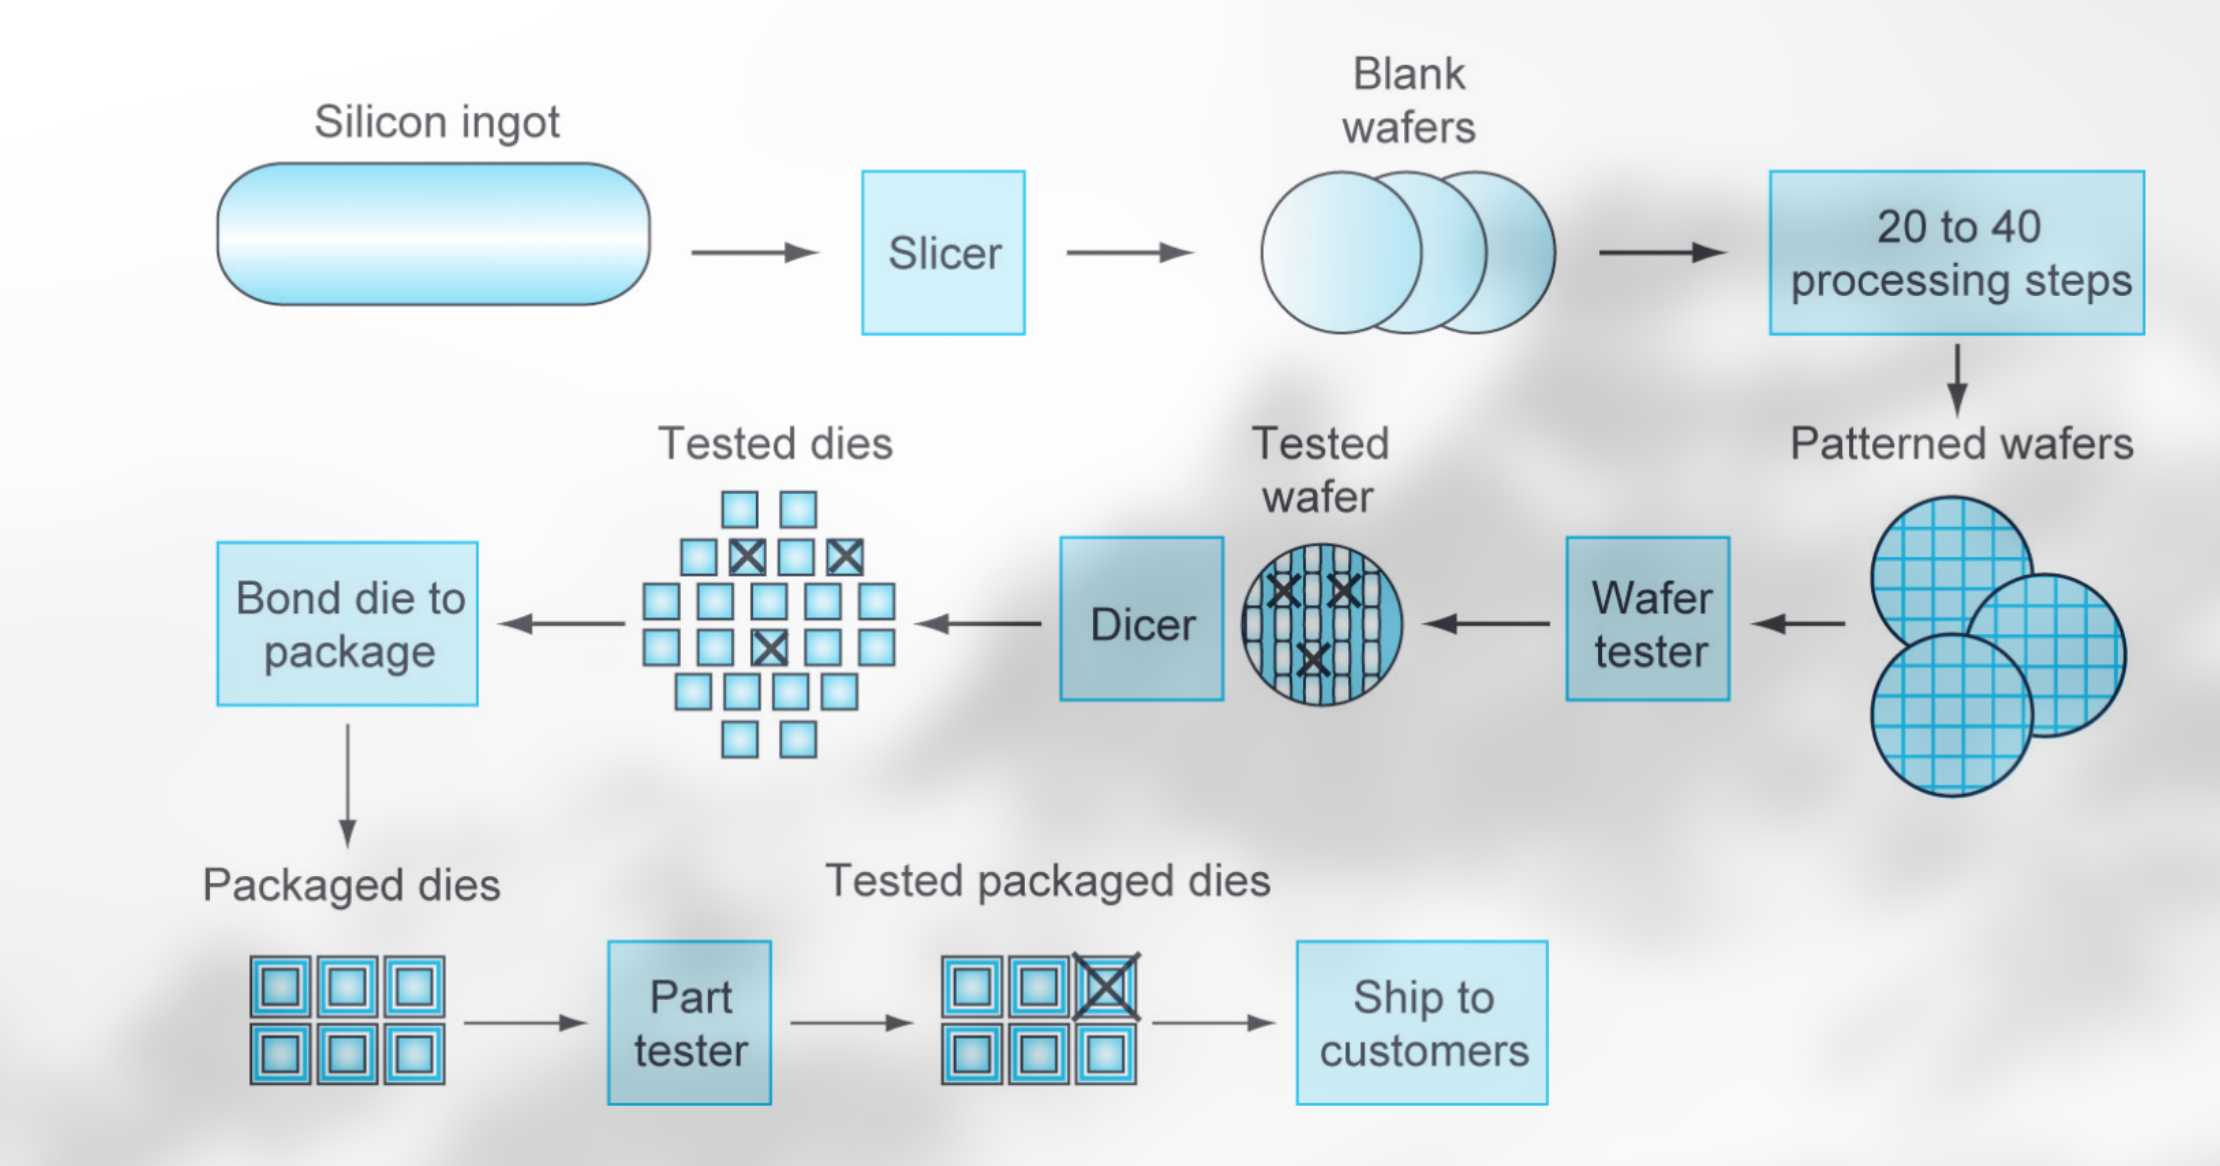
\includegraphics{images/silicon.png}
    \caption{Silicon Lifecycle}
    \label{fig:silicon}
\end{figure}
The faulty chips that fail to meet speed benchmarks
are sold as lower-grade chips in a process termed
\emph{binning}.

Even the simplest modern computers take thousands
of engineers to design. It isn't feasible to
understand everything about a computer at every
level, so we must abstract and think of the system
in terms of black boxes with inputs and outputs. This
applies to electrical engineering, computer engineering,
and programming. A high-level language like Python is
an abstraction of C, which is an abstraction of assembly
language, which is an abstraction of binary machine language.
\begin{lstlisting}[language=C]
    // Consider the C statement
    f = (g + h) - (i + j);
    // The corresponding 
    // assembly could be
    add t0, g, h  // t0 = g + h
    add t1, i, j  // t1 = j + j
    sub f, t0, t1 // f = t0 - t1
    // The corresponding machine 
    // instruction would be 0s 
    // and 1s
\end{lstlisting}
The assembly code corresponding to a given statement in
C depends on the device. Devices may run x86, ARM, or RISC-V,
which are known as \emph{instruction set architectures} (ISAs).
There are three different types of ISAs:
\begin{itemize}
    \item CISC (Complex Instruction Set Computer)
    \item RISC (Reduced Instruction Set Computer)
    \item DSPs (Digital Signal Processors)
\end{itemize}
In this class we focus on RISC, specifically RISC-V.

The general instruction cycle for what a computer is doing under the
hood is:
\begin{enumerate}
    \item Fetch: retrieve the next instruction from memory.
    \item Decode: figure out what the instruction needs to do
          by determining what operations and additional operands
          are required for execution and sends respective signals
          to respective components within the CPU, such as the ALU
          or FPU, to prepare for the execution of the instruction.
    \item Execute: the stage where the actual operation
          specified by the instruction is carried out by the relevant
          functional units of the CPU. Logical or arithmetic operations
          may be run by the ALU, data may be read from or written to
          memory, and the results are stored in registers or memory as
          required by the instruction. Based on output from the ALU,
          the PC might branch.
    \item Update PC: point the program counter at the next instruction.
\end{enumerate}
All CPUs use a pipeline, which could have as few steps as these four
steps or as many as twelve.